\documentclass[11pt]{article}
\usepackage[a4paper,left=2.5cm,right=2.5cm,top=\dimexpr15mm+1.5\baselineskip,bottom=2cm]{geometry}
\usepackage[english]{babel}
\usepackage[T1]{fontenc}
\usepackage[utf8]{inputenc}
\usepackage{geometry}
\usepackage{fancyhdr} % Headings
\usepackage{listings} % Code
\usepackage{parskip} % Spacing for Paragraphs
\usepackage{mdframed} % Asides
\usepackage{caption}
\usepackage{graphicx}
\usepackage{amsmath}

% Asides
\newenvironment{aside}
  {\begin{mdframed}[style=0,%
      leftline=false,rightline=false,leftmargin=2em,rightmargin=2em,%
          innerleftmargin=0pt,innerrightmargin=0pt,linewidth=0.75pt,%
      skipabove=7pt,skipbelow=7pt]\small}
  {\end{mdframed}}

\renewcommand{\headrulewidth}{.2mm} % header line width


\newcommand{\myeq}[1]{
    \vspace{11pt}
    \begin{center}
        ${#1}$
    \end{center}
    \vspace{11pt}
}

\newcommand{\myeqfol}[1]{
    \begin{center}
        ${#1}$
    \end{center}
    \vspace{11pt}
}

\newcommand{\img}[2][0.6]{
    \vspace{11pt}
    \begin{center}
        \includegraphics[width=#1\textwidth]{#2}
    \end{center}
    \vspace{11pt}
}

\newcommand{\topsec}[1]{
    \vspace{11pt}
    \section{#1}
    \vspace{11pt}
}

\newcommand{\boldsec}[1]{
    \vspace{11pt}
    \textbf{#1}
    \vspace{11pt}
}


\newcommand{\boldsecbottom}[1]{
    \textbf{#1}
    \vspace{11pt}
}

\rhead{\today}
\lhead{\textbf{Maxwell Klema}}
\cfoot{\thepage}


\title{Analysis of Algorithms}
\date{Spring 2026, Purdue University Fort Wayne}
\author{Maxwell Klema | Professor Zesheng Chen}

\lstset{
    frame=single, % Adds a single line frame around the code
}

\begin{document}

\maketitle
\pagestyle{fancy}


% The well known Pythagorean theorem \(x^2 + y^2 = z^2\) was 
% proved to be invalid for other exponents. 
% Meaning the next equation has no integer solutions:

% \[ x^n + y^n = z^n + log(n)\]
% \[\sqrt{x^2+1}\] 
% This is a simple math expression \(\sqrt{x^2+1}\) inside text. 
% And this is also the same: 
% \( \log_b a\)
% \begin{lstlisting}[language=Python]
%     dsad
% \end{lstlisting}


\section{Lecture 1 - Algorithms Introduction}
\vspace{11pt}
\textbf{Merge Sort} is sort of like the "hello world" for advanced algorithms. In a merge sort, you keep splitting the array in half until there are only chunks of one element, then you merge back up. This means that you take two single elements and merge them from smallest to largest. Then, you take that shorted chunk of some size \textit{m}, and merge it with another sorted array of some size \textit{m}, until the whole array with \textit{n} elements is sorted.

A good example to try a merge sort on is \textit{[5, 4, 1, 8, 7, 2, 6, 3]}.

\vspace{11pt}
\subsection{Why Study Algorithms?}
\vspace{11pt}

\textbf{Review: What is an Algorithm?} It's a set of well-defined rules - a recipe, in effect - for solving some computation problem.

Example: Sorting, shortest path, and scheduling.

It is important to study algorithms because it applies to all other branches of computer science. For example, in Networking, there are routing protocols such as Dijkstra's algorithm. There is intra-domain and inter-domain routing which may use different routing algorithms. In Computer Security, there are many cryptography algorithms. In Computer Graphics, there are geometric algorithms. In databases, there are balance search tree algorithms to speed up database queries using indexing. In Computational Biology, dynamic programming is heavily used. In Machine Learning, any model, including deep learning models, is a set of algorithms. An example is a clustering algorithm.

Studying algorithms plays a key role in modern technological innovation.
\vspace{11pt}
\begin{aside}
"Everyone knows Moore's Law - a prediction made in 1965 by Intel c-ofounder Gordon Moore that the density of transistors in integrated circuits would continue to double every one to two years... in many areas, performance gains due to improvements in algorithms have vastly exceeded even the dramatic performance gains due to increased processor speed."

- Excerpt from Report to the President and Congress: Designing a Digital Future, December 2010 (page 71).
\end{aside}
\vspace{11pt}
Another famous use-case of algorithms is Google's PageRank algorithm, which measures the "quality" of a webpage based on how many other pages refer to it, as well as other quality metrics. This algorithm relies on probability distribution using eigenvectors and matrices.

Additionally, studying algorithms provides a novel "lens" on processes outside of computer science and technology. This includes quantum mechanics, economic markets, and evolution.

Studying algorithms is also challenging. But, that makes you a better programmer and an overall better problem-solver. It can also be fun: seeing an abstract problem and coming up with a creative solution. It is the blend of precision and creativity.

\subsection{Integer Multiplication and Karatsuba}
\vspace{11pt}
\subsubsection{Integer Multiplication Problem}
\textbf{Input}: 2 n-digit numbers $x$ and $y$.

\textbf{Output}: product of $x * y$.
\vspace{11pt}
\\A "primitive operation" may be adding or multiplying 2 single-digit numbers, and adding a zero to the beginning or end of a number.

For example, $12 + 8$ takes two operations: $8 + 2$ and $1 + 1$.


\vspace{11pt}
\textbf{The Grade-School Algorithm}
\vspace{11pt}

Let's calculate $5678 * 1234$. Because it is O(\(6n^2\)) (double-check), it should take a maximum of \texttt{\~}96 operations to solve.

\vspace{11pt}
\begin{aside}
    \textbf{Note}: To get O(\(6n^2\)), it is important to understand the the multiplication phase takes O(\(3n^2)\) operations (the multiply, the addition of the carry from the previous digit in the same row, and the update that calculates the new carry to pass to the new digit to the left). The addition phase, similarly, takes O(\(3n^2\)) operations (the addition in the column, the addition of the carry-in that came from the column to the right, and the calculation of the carry-out to the column on the left).
\end{aside}
\vspace{11pt}

However, that is pretty bad. Can we do better than the "obvious" or "bruteforce" method?

What if we take a divide-and-conquer approach? We divide each number into half and then half and then half, i.e. recursively divide n-digit number into half until it is a single digit and then merge it back into the actual solution.

For example, a = 56, b = 78, c = 12, d = 34. 

Let $x = {10^{n/2}} * a + b$. 

Let $y = {10^{n/2}} * c + d$. 

Finally, $x * y = ({10^n} * ac) + {10^{n/2}}(ad+bc) + bd$

$x*y$ contains $\{ac, ad, bc, bd\}$. These four items are still integer multiplication. For each of these, you apply $x * y$ and get another $4$ items (like a tree). Then you merge them back.

n $\to$ {n/2} $\to$ {n/4} $\to$ ... $\to$ {1 digit}

However, this algorithm does not do better! Why? Because, eventually, the time complexity is O(\(n^2\)).
\vspace{11pt}
\begin{aside}
    The recursive relation of the problem can be expressed as $T(n) = 4T({n/2}) + O(n)$, where O(n) is the work needed to "merge" the results (adding the products and shifting digits by adding zeros). Four is the number of smaller multiplications to perform, while {n/2} shows that each of the smaller multiplications deals with numbers half the size of the original.

    \(log_24 = 2\) shows that each additional level does 2 times more work. By the time you reach 1-digit numbers, you perform exactly \(n^2\) multiplications - the same as grade-school.

    Therefore, O(\(n^{log_24})\) = O(\(n^2)\).
\end{aside}
\vspace{11pt}
\subsubsection{Karatsuba Multiplication}

So, how does Karatsuba Multiplication fix this?

(a+b)*(c+d) = ac + ad + bc + bd, then subtract - ac - bd = ad + bc. \textbf{You can reduce four recursive calls into three}. That's certaintly better than third-grade multiplication.

The three recursive calls are: $ac$, $bd$, $(a+b) * (c+d)$, then $sum(ad + bc)$ becomes the third.

The new recursive formula becomes:

$T(n) = 3T({n/2) + O(n)}$

Thus, the new additional work factor is only \(log_23 = 1.58\), showing that each level does 1.58 times more additional work than the last, making the overall time complexity \textbf{O(\(n^{log_23})\)}.

For large n-digit multiplications, they use Karatsuba Multiplication.

\vspace{11pt}
\subsection{Merge Sort}

Merge sort is a good introduction to divide-and-conquer algorithms. It improves over selection, insertion, and bubble sorts. These are all O(\(n^2\)).

It helps to calibrate your preparation and motivates guiding principles for algorithm analysis (worst-case and asymptotic analysis).

Analysis generalizes to "Master Method".

\subsubsection{The Sorting Problem}

\textbf{Input:} array of n numbers, unsorted.

\textbf{Output:} Same numbers, sorted in increasing order.
\vspace{11pt}
\begin{aside}
    \textbf{Note}: For now, we assume that all elements are distinct.
\end{aside}
\vspace{11pt}
\subsubsection{Merge Sort: Example}
\vspace{11pt}
\textit{[5,4,1,8,7,2,6,3]} $\to$ \textit{[5,4,1,8] \& [7,2,6,3]} $\to$ ... (recursion) ... $\to$ \textit{[1,4,5,8] \& [2,3,6,7]} $\to$ \textit{[1,2,3,4,5,6,7,8]}

\vspace{11pt}
\subsubsection{Merge Sort: Pseudocode}

Three function calls: Recursively sort 1st half of the input array, recursively sort 2nd half of the input array, and merge two sorted sublists into one.

The base case for merge sort is when there is only one element or there are zero elements (where n \% 2 != 0).

C = output[length = n]

A = 1st sorted array [n/2]

B = 2nd sorted array [n/2]

i = 1
\\
j = 1
\vspace{11pt}
\begin{aside}
    \textbf{Note:} we assume the starting point is 1 instead of 0.
\end{aside}
\vspace{11pt}

\begin{lstlisting}[language=Python]
for k = 1 to n  
    if A(i) < B(j)
        C(k) = A(i)
        i++
    else [B(j) < A(i)]
        C(k) = B(j)
        j++

\end{lstlisting}
\vspace{11pt}
\vspace{11pt}
\begin{aside}
    \textbf{Note:} This is just the pseudo code for merging, which is O(m). Where m $\leq$ n.
\end{aside}
\vspace{11pt}

\textbf{Running Time of Merge Sort}
\vspace{11pt}

The time complexity is O(\(nlog(n)\)). It takes \(log_2n\) times to divide an array of size n by 2 to get 1 or 0 elements.

The running time is roughly \# amount of lines of code executed.

\textbf{Upshot:} the running time of \textbf{merge} in the array of m numbers is 4m + 2 $\leq$ 6m where m $\geq$ 1

\textbf{Claim:} Merge Sort requires $\leq$ \(6n*log_2n + 6n\)  operations to sort n numbers

\vspace{11pt}
\begin{aside}
    \textbf{Recall:} \(log_2n\) is the \# of times you divide by 2 until you get down to 1.
\end{aside}
\vspace{11pt}

\textbf{Proof of claim (assuming n = power of 2)}

Use a recursive tree:

level 0 $\to$ root (outer call to Merge Sort) [\(2^1 - 1 = 1\) cumulative divisions]

level 1 $\to$ 1st recursive call [\(2^2 - 1 = 3\) cumulative divisions]

level 2 $\to$ 2nd recursive call [\(2^3 - 1 = 7\) cumulative divisions]

...

\vspace{11pt}
\begin{aside}
   \textbf{Quiz:} Roughly how many levels does this recursion tree have (as a function of $n$, the length of the input array)?

   $\to$ \(log_2n\), well actually \(log_2n + 1\) for the root level.
\end{aside}
\vspace{11pt}

\vspace{11pt}
\begin{aside}
   \textbf{Quiz:} What is the pattern? Fill in the blanks in the following statement: at each level j = 0,1,2,.., \(log_2n\), there are <blank> subproblems, each of size <blank>.

   $\to$ \(2^j\) subproblems \& each the size of \(n / 2^j\).

   \textbf{Proof of claim (assuming n = power of 2):} 
   
   $\leq$ \(2^j * 6(n/2^j) = 6n\), where $6$ is the work per level-j subproblem.

   If there is $6n$ work per level, and there are \(log_2n + 1\) levels, then the total Big-O time complexity is:

   O(\(6n(log_2n + 1)\))
\end{aside}
\vspace{11pt}

\subsection{Guiding Principles for Analysis of Algorithms}
\vspace{11pt}
\textbf{Guiding Principle \#1}
\vspace{11pt}

"Worst-case analysis": Our running time bound holds for every input of length n. This is particularly appropriate for "general-purpose" routines, as opposed to "average-case" analysis and benchmarks.

In fact, the worst-case analysis is usually easier to analyze, making our job easier.

\vspace{11pt}
\textbf{Guiding Principle \#2}
\vspace{11pt}

Constant factors and lower-order terms do not need to be paid much attention to. The justifications for this include making algorithms easier to analyze, the fact that constants depend on architecture, compiler, and/or programmer anyways, and that the reduction of constants lose only very little predictive power (as we will see).

\vspace{11pt}
\textbf{Guiding Principle \#3}
\vspace{11pt}

\textbf{Asymptotic Analysis:} Focus on running time for large input size $n$.

\vspace{11pt}
\begin{aside}
    \textbf{For example}: \(6nlog_2n + 6n\) [merge sort] may be worse than \((1/2)n^2\) [insertion sort] for very small n. This can lead to wrong conclusions that insertion sort is better, but at a small enough n, the difference in performance is extremely minimal (nanoseconds).
\end{aside}
\vspace{11pt}

Really, only big problems with large n are interesting, as different Big-O functions involving n have different growth rates.

\vspace{11pt}
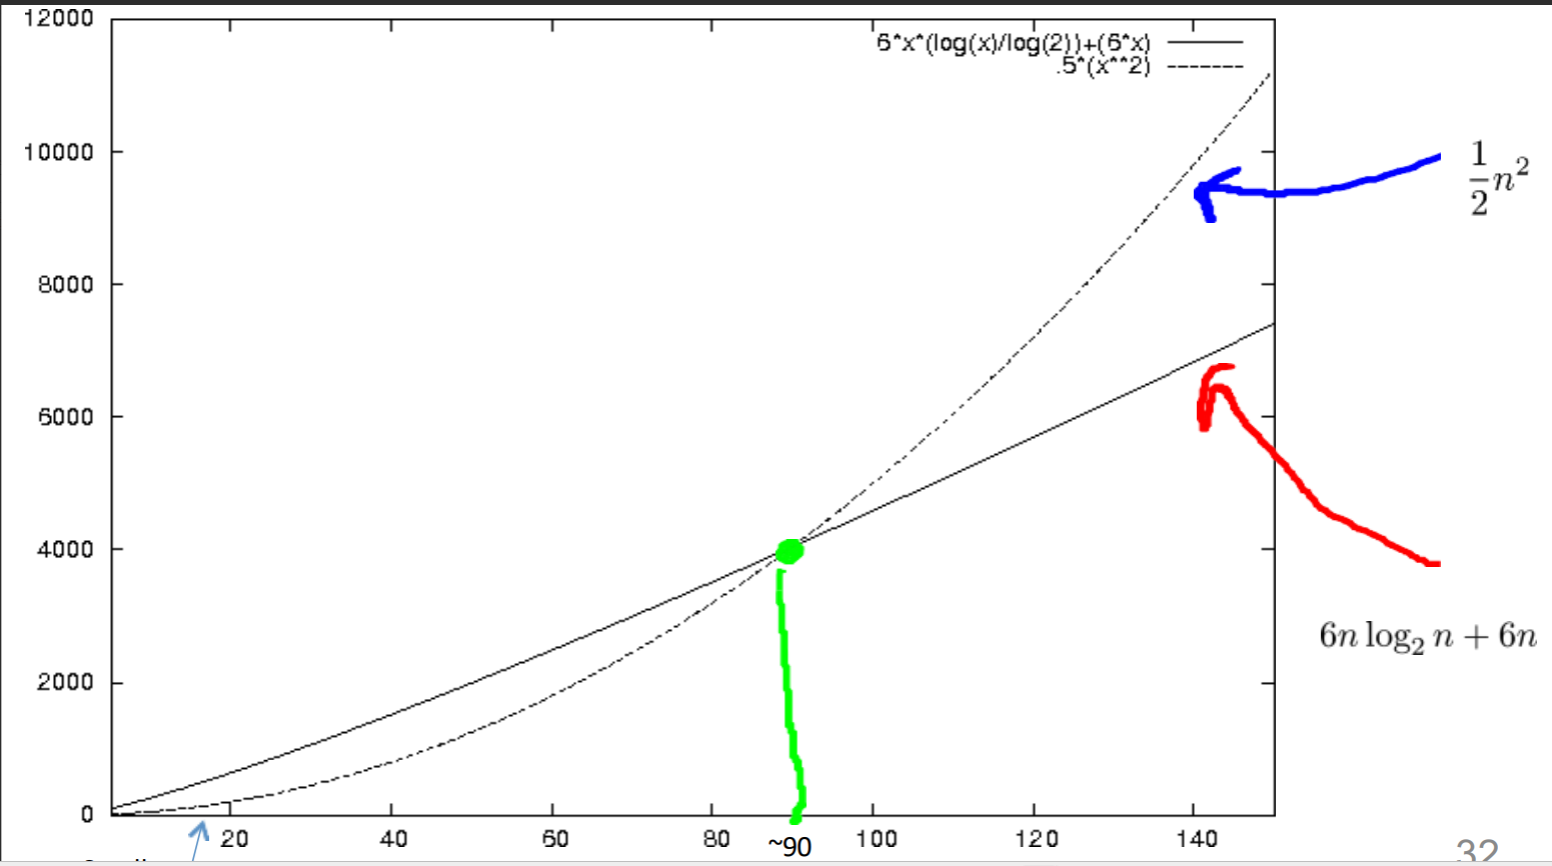
\includegraphics[width=0.7\textwidth]{1.png}

\vspace{11pt}
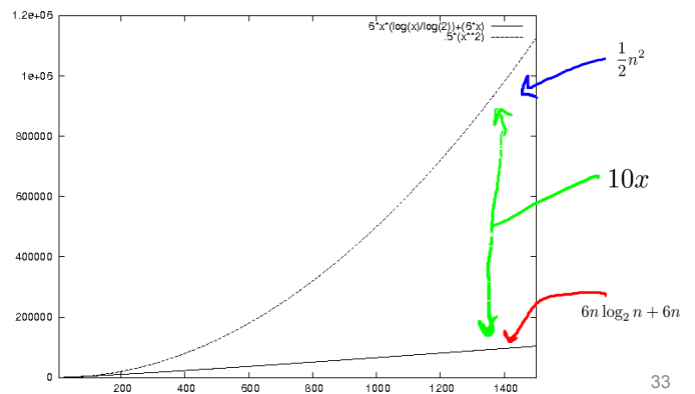
\includegraphics[width=0.7\textwidth]{2.png}

\vspace{11pt}
\textbf{What is a "Fast" Algorithm?}
\vspace{11pt}

A fast algorithm is one where the worst case running time grows slowly with input size. An example being O(\(log_2n\)) or even O(1), although that is rare.

\vspace{11pt}
\begin{aside}
    A good goal is usually keeping an algorithm as close to \(O(n)\) as possible.
\end{aside}
\vspace{11pt}

\vspace{11pt}
\textbf{For-Free Primitives}
\vspace{11pt}

An algorithm with a linear or near-linear running time acts as a primitive that can be used essentially "for free". In other words, the amount of time required barely exceeds what you need to read the input.

An example of this can be sorting. It is important to put these for-free primitive algorithms into your toolbox.

\newpage
\section{Lecture 2 - Asymptotic Notation}
\vspace{11pt}

In the last lecture, we talked about the Integer multiplication problem (x*y). However, using traditional methods, for an n-digit number, the runtime is O($n^2$). Can we do better?

Can we use divide-and-conquer? What about $n/2 \to n/4 \to ...\to 1$.

For example, say $x=5678, y=1234$, then cut in half such that $a=56,b=78,c=12,d=34$.

Then, $x=100a+b, y=100c+d$

$x*y=(100a+b)(100c+d)$.

$= 10^4ac + 100ad + 100bc + bd$. Now, given this, we are turning this into 4 $n/2$ digit product. We can keep going recursively by dividing in half. However, this does not make life easier. In fact, the running time complexity is still $O(n^2)$.

If we look at $(a+b)(c+d)=ac+ad+bc+bd$. We can get $(ad+bc)$ using $ac+ad+bc+bd - ac - bd = ad+bc$. Now, instead of four operations per level, we can do three operations instead. It is 3 $n/2$ digit multiplication. This does better than the elementary school multiplication algorithm.

\vspace{11pt}
\subsection{Merge Sort}
\vspace{11pt}

We then began talking about \textbf{Merge Sort}. Given an array, we split the array in half and then recursively sort both halves. Once both halves are sorted, we then merge them together.

If we assume that there are $m$ total elements in the array, and each half has $m/2$ elements. For the merge, $2m \geq 2$ and the time complexity is $\leq 4m + 2m = 6m$.

In a recursive tree, we divide each node into two sub-arrays until we have single-element arrays. Each level has $2^j$ nodes per level. There are $n$ nodes at the end. Given that $j = log_2n$, then there are $log_2n+1$ levels. For each node (sub-array), there are $n/2^j$ nodes.

Then, for each level there are $n/2^j * 6 * 2^j$ steps. With $log_2n+1$ levels, the overall runtime complexity is $O(6nlog_2n + 6n)$.

\vspace{11pt}
\subsection{Asymptotic Notation}
\vspace{11pt}

The goal is to identify a sweet spot of granularity for reasoning about algorithms. We want to suppress second-order details like constant factors and lower-order terms and introduce Big-O notation.

In seven words, asymptotic notation \textbf{suppresses constant factors and lower-order terms}. Constant factors are too system-dependent. For example, a programming language, architecture, or compiler. Additionally, lower-order terms are irrelevant for large inputs. For example, having $3n^2+2n$, we can just write it as $O(n^2)$. The "big-O notation" buckets algorithms into groups according to their asymptotic worst-case running time.

\vspace{11pt}
\textbf{Examples:}

Input: array A of n integers, and an integer t. Output is whether or not A contains t. $\to$ $O(n)$

Input: arrays A and B of n integers each, and an integer t. The output whether or not A or B contains t. $\to$ $O(n)$

Input: arrays of A and B of n integers each. Output: Whether or not there is an integer t contained in both A and B. $\to$ $O(n^2)$

Input: an array of A of n integers. Output: Whether or not A contains an integer more than once. Note, assume that we are using two for loops. $\to$ $O(n^2)$. Another way is $n$ choose $2$ permutations which equates to $\frac{n(n-1)}{2}$.

\vspace{11pt}
\subsection{Big-O Notation [Asymptotic Upper Bound]}
\vspace{11pt}

Let $T(n)=$ function on $n = 1, 2, 3, ...$ [usually, the worst-case running time of an algorithm, or the real running time of an algorithm]. A big question is \textbf{when is $T(n)=O(f(n))$?} If eventually (for all sufficiently large $n$), $T(n)$ is bounded above by a constant multiple of $f(n)$.

In other words, $O(f(n))$ is a way to categorize or "bound" the runtime. It describes the "shape" of the growth as $n$ becomes very large.
\vspace{11pt}

The formal definition states that $T(n)=O(f(n))$ if and only if there exists constants such that $c, n_0 > 0$:

\vspace{11pt}
\begin{center}
    $T(n) \leq c * f(n)$
\end{center}
\vspace{11pt}

for all $n \geq n_0$. Also $c, n_0$ cannot depend on $n$.

\vspace{11pt}
\begin{aside}
    \textbf{Note:} $c$ is the constant multiple (positive) that scales the function $f(n)$. Its purpose allows us to ignore specific implementation details like hardware speed or compiler optimizations. It matters because even if an algorithm takes $3n^2$ steps, we can say it is $O(n^2)$ because we can just pick $c=3$ (or any higher number) to satisfy the inequality. It focuses on the analysis on the rate of growth rather than the exact number of operations.

    Meanwhile, $n_0$ is the threshold or starting point. It is the value of the input size $n$ where the upper bound starts to kick in. Big-O notation is interested in asymptotic behavior, meaning what happens as $n$ grows to infinity. For very small inputs, an algorithm might be slow due to initialization or overhead (e.g., 100 + n is larger than $n^2$ when $n=2$). The $n_0$ value says to ignore those small cases. Eventually, $c*f(n)$ will always be greater than or equal to $T(n)$ for every value of $n$ from this point onward.
\end{aside}
\vspace{11pt}

\textbf{A Picture Illustrating When $T(n)=O(f(n))$}

\vspace{11pt}
\begin{center}
    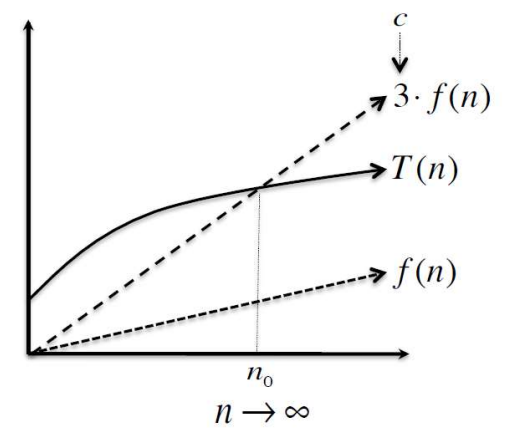
\includegraphics[width=0.5\textwidth]{3.png}
\end{center}
\vspace{11pt}

\newpage
Note, in the image above, $3*f(n)$ is used as an upper bound to show that $T(n)=O(f(n))$.

\vspace{11pt}
\textbf{Example 1:}

Claim: If $T(n)=a_kn^k+\dots+a_1n+a_0$, then $T(n)=O(n^k)$

Proof: Choose $n_0=1$ and $c=|a_k| + |a_{k-1}| + \dots + |a_1| + |a_0|$. We need to show that $\forall n \geq 1,T(n) \leq c*n^k$.

We have, for every $n \geq 1$:

\vspace{11pt}
\begin{center}
$T(n) \leq |a_k|n^k + \dots + |a_{1}|n+|a_0|$

$\leq |a_k|n^k + \dots + |a_1|n^k + |a_0|$

$= c*n^k$
\end{center}

\vspace{11pt}
\textbf{Example 2:}

Claim: For every $k \geq 1$, $n^k$ is not $O(n^{k-1})$

Proof: By contradiction. Suppose $n^k=O(n^{k-1})$. Then, there exists constants $c,n_0$ such that:

\vspace{11pt}
\begin{center}
    $n^k \leq c*n^{k-1}$ for $\forall n \geq n_0$

    But then [canceling $n^{k-1}$ from both sides]:

    $n \leq c$ for $\forall n \geq n_0$

    Which is clearly false [Contradiction]
\end{center}

\vspace{11pt}
\textbf{Example 3:}

Claim: $2^{n+10}=O(2^n)$

Proof: We need to pick constants $c,n_0$ such that:

\vspace{11pt}
\begin{center}
    (*) $2^{n+10} \leq c * 2^n$ for $\forall n \geq n_0$

    Note: $2^{n+10}=2^{10}*2^n=(1024)*2^n$.
\end{center}
\vspace{11pt}

So, if we choose $c \geq 1024,n_0=1$, then (*) holds.

\vspace{11pt}
\textbf{Example 4:}

Claim: $2^{10n} \neq O(2^n)$

Proof: By contradiction, if $2^{10n}=O(2^n)$ then there exist constants $c,n_0 > 0$ such that:

\vspace{11pt}
\begin{center}
    $2^{10n} \leq c*2^n$ for $n \geq n_0$

    But then [canceling $2^n$]:

    $2^{9n} \leq c$ for $\forall n \geq n_0$,

    which is certainly false.
\end{center}
\vspace{11pt}

\newpage
\subsection{Big-Omega Notation [Asymptotic Lower Bound]}
\vspace{11pt}

The formal definition is $T(n)=\Omega(f(n))$ if and only if there exists constants $c,n_0 > 0$ such that:

\vspace{11pt}
\begin{center}
    $T(n) \geq c *f(n)$ for $\forall n \geq n_0$
\end{center}
\vspace{11pt}

In other words, the inequality $T(n) \geq c * f(n)$ means that for all sufficiently large inputs $(n \geq n_0)$, the actual runtime $T(n)$ will always be greater than or equal to a constant multiple of $f(n)$. This implies that the algorithm will never run faster than that bound once the input size is large enough.

Again, $c,n_0$ cannot depend on $n$.

\vspace{11pt}
\subsection{Big-Theta Notation [Asymptotic Tight Bound]}
\vspace{11pt}

The formal definition is $T(n)=\theta(f(n))$ if and only if there exist constants $c_1,c_2,n_0$ such that:

\vspace{11pt}
\begin{center}
    $c_1*f(n)\leq T(n) \leq c_2 *f(n)$ for $\forall n \geq n_0$
\end{center}
\vspace{11pt}

In other words, $T(n)=\theta(f(n))$ does not specify an average running time, but rather a tight bound for whatever runtime function $(T(n))$ is being analyzed. $c_1*f(n)$ acts as the lower bound (the floor): The function cannot grow any slower than this. Meanwhile, $c_2*f(n)$ acts as the upper bound (ceiling): The function cannot grow any faster than this.

Again, $c_1,c_2,n_0$ cannot depend on $n$.

Mean: $T(n)=O(f(n))$ ($(T(n)$ does not grow faster than $f(n)$) and $T(n)=\Omega(f(n))$ ($T(n)$ does not grow slower than $f(n)$).

\vspace{11pt}
\textbf{A Quiz}
\vspace{11pt}

Let $T(n)=\frac12n^2+3n$. Which of the following statements are true? (There might be more than one correct answer.)
\begin{itemize}
    \item $T(n)=O(n)$. False! $\frac{1}{2}n+3 \not\leq c$.
    \item $T(n)=\Omega(n)$. True! $\frac12n+3 \geq c$. A quadratic function always grows faster than a linear one. Therefore, the quadratic function will always be "at least" as large as a linear function for large values of $n$, $n^2$ is bounded below by $n$.
    \item $T(n)=\Theta(n^2)$. True! $c_1 \leq \frac12+\frac3n \leq c_2$. To prove this, $T(n)=\Omega(n^2),T(n)=O(n^2)$.\textbf{ The function must satisfy the function using the same $f(n)$.}
    \item $T(n)=O(n^3)$. True! $\frac12+\frac3n \leq c*n$.
\end{itemize}
\vspace{11pt}

\textbf{Example on Big-Theta Notation}

Claim: for every pair of positive function $f(n)$ and $g(n)$:

\vspace{11pt}
\begin{center}
    $\max\{f,g\}=\theta(f(n)+g(n))$
\end{center}
\vspace{11pt}

Proof: For every $n$, we have:

\vspace{11pt}
\begin{center}
    $\max\{f(n),g(n)\} \leq f(n)+g(n) $
\end{center}
\vspace{11pt}

and

\vspace{11pt}
\begin{center}
    $2*\max\{f(n),g(n)\} \geq f(n)+g(n) = \max\{f(n),g(n)\} \geq \frac12(f(n)+g(n))$
\end{center}
\vspace{11pt}

Thus

\vspace{11pt}
\begin{center}
    $\frac12 * (f(n)+g(n)) \leq \max\{f(n),g(n)\} \leq f(n)+g(n)$ for $\forall n > 1$

    $=> \max\{f,g\} = \theta(f(n)+g(n))$ [where $n_0=1,c_1=\frac12,c_2=1$]
\end{center}
\vspace{11pt}

\textbf{Little-O Notation [Mathematical Version]}
\vspace{11pt}

Definition: $T(n)=o(f(n))$ if and only if \textbf{for all} constants $c>0$, there exists a constant $n_0$ such that:

\vspace{11pt}
\begin{center}
    $T(n) \leq c * f(n)$ for $\forall n \geq n_0$
\end{center}
\vspace{11pt}

Exercise: $\forall k \geq1,n^{k-1}=o(n^k)$. Simplifying both sides yields $1 \leq c*n$. This showcases little-o since for any constant $c>0$, the inequality still holds.

\vspace{11pt}
In asymptotic notation, Big-O and little-o both describe upper bounds, but with different strength.

Big-O --- Grows as most as fast as (allowing the same growth rate)

Little-o --- grows strictly slower than (must be asymptotically smaller).

Therefore, Little-o is a much stronger upper-bound than big-O.

\vspace{11pt}
\textbf{Where does Notation Come From?}
\vspace{11pt}

"On the basis of the issues discussed here, I propose that members of SIGACT, and editors of computer science and mathematics journals, adopt the $O,\Omega,\Theta$ notations as defined above, unless a better alternative can be found reasonably soon". --- \textit{D.E. Knuth, 
"Big Omicron and Big Omega and Big Theta", SIGACT News, 1976. Reprinted in "Selected Papers on Analysis of Algorithms"}

\vspace{11pt}
\textbf{Summary}
\vspace{11pt}

It is important to remember asymptotic notation in seven words: "Suppress constant factors and lower-order terms." It is important to understand Big-O, Big-Omega, Big-Theta, and Little-O Notations.

It should also be a goal to understand how to find constants to show Big-O and to understand how to apply contradiction to show not Big-O.

\newpage
\section{Lecture 3 - Divide and Conquer}
\vspace{11pt}

The goal is to provide practice with the divide-and-conquer algorithm design paradigm through applications to two basic problems.

\vspace{11pt}
\subsection{Divide-and-Conquer Paradigm}
\vspace{11pt}

The overall goal of the divide-and-conquer paradigm is to divide the input into smaller subproblems. The next step is to conquer the subproblems recursively, and finally, to combine the solutions for the subproblems into a solution for the original problem.

An example is Merge Sort.
\begin{itemize}
    \item 1) Divide: Splits the input array into its left and right halves.
    \item 2) Conquer: Uses two recursive calls to sort the left and right sub-arrays.
    \item 3) Combine: Implemented by the Merge subroutine.
\end{itemize}
\vspace{11pt}

\textbf{When to Apply the Divide-and-Conquer Paradigm?}

\vspace{11pt}
In general, this design paradigm is well-suited to computational problems for which there is an obvious way to split the input into smaller subproblems that do not interfere with each other.

\vspace{11pt}
\subsection{Counting Inversions}
\vspace{11pt}

Input: array A containing the numbers $1, 2, 3, \dots, n$ in some arbitrary order.

Output: \textbf{number of inversions = number of pairs $(i,j)$ of array indices with $i<j$ and $A[i]>A[j]$}.

For example, given an array $[1,3,5,2,4,6]$: there are three inversions: $(3,2), (5,2), (5,4)$.

\vspace{11pt}
\textbf{Quiz:} What is the largest possible number of inversions that a 6-element array can have?
\vspace{11pt}

$\to$ Assuming a completely unsorted array like $[6,5,4,3,2,1]$, the maximum number of inversions is given by 6 choose 2, or $\binom{n}{2} = \frac{n!}{r!(n-r)!}$. Therfore, $\binom{6}{2} = \frac{6!}{2!(6-2)!} = 15$.

Note: permutations is not used because that counts every possible pair, which may include $(i,j)$ that are not inversions. Therefore, we do not care about order, so combinations are used.

\vspace{11pt}
\textbf{Why Study This Problem?}
\vspace{11pt}

One reason is to compute a numerical similarity measure that quantifies how close two ranked lists are to each other. Another is collaborative filtering: a technique for generating recommendations. 

The smaller number of inversions, the more similar the rankings: $0 \leq \# \leq \binom{n}{2} = \frac{n(n-1)}{2}$.x

\vspace{11pt}
\textbf{Different Ways of Finding the Number of Inversions}
\vspace{11pt}

A naive approach would be an exhaustive search for counting inversions in $O(n^2)$ running time.

Input: Array A of n distinct integers.
Output: the number of inversions of A.

\vspace{11pt}
\begin{lstlisting}
numInv := 0
for i := 1 to n - 1 do
    for j := i + 1 to n do
        if A[i] > A[j] then
            numInv := numInv + 1
return numInv
\end{lstlisting}
\vspace{11pt}

A \textbf{Divide-and-Conquer Approach} is similar to the MergeSort algorithm, with one recursive call for the left half of the array and the other for the right half. There are three types of inversions
\begin{itemize}
    \item Left inversion: an inversion with $i,j$ both in the first half of the array (i.e, $i,j < \frac{n}{2}$).
    \item Right inversion: an inversion with $i,j$ both in the second half of the array (i.e., $i,j > \frac{n}{2}$).
    \item Split inversion: an inversion with $i$ in the left half and $j$ in the right half (i.e., $i \leq \frac{n}{2} \leq j$).
\end{itemize}
\vspace{11pt}

A high-Level Algorithm of this is \texttt{CountInv}.

Input: array A of $n$ distinct integers.

Output: the number of inversions in A

\vspace{11pt}
\begin{lstlisting}
if n = 0 or n = 1 then
    return 0
else
    leftInv := CountInv(first half of A)
    rightInv := CountInv(second half of A)
    splitInv := CountSplitInv(A)
    return leftInv + rightInv + splitInv
\end{lstlisting}
\vspace{11pt}

A key idea is having the recursive calls both count inversions and sort [i.e., piggyback on MergeSort]. The motivation for this is that the merge subroutine naturally uncovers split inversions as we will see.

To revise this High-Level Algorithm, we include the \texttt{Sort-and-CountInv} algorithm.

Input: array A of $n$ distinct integers.

Output: sorted array B with the same integers, and the number of inversions of A.

\vspace{11pt}
\begin{lstlisting}
if n = 0 or n = 1 then //base case
    return (A, 0)
else
    (C, leftInv) := Sort-and-CountInv(first half of A)
    (D, rightInv) := Sort-and-CountInv(second half of A)
    (B, splitInv) := Merge-and-CountSplitInv(C,D)
    return (B, leftInv + rightInv + splitInv)
\end{lstlisting}
\vspace{11pt}

It is important to re-visit the \texttt{merge} sort algorithm.

Input: sorted Arrays C and D (length $n/2$ each)

Output: Sorted Array B (length $n$)

\vspace{11pt}
\begin{lstlisting}
i := 1, j := 1
for k := 1 to n do
    if C[i] < D[j] then
        B[k] := C[i], i := i + 1
    else // D[j] < C[i] (inversion)
        B[k] := D[j], j := j + 1
\end{lstlisting}
\vspace{11pt}

\textbf{Quiz:} Suppose the input array $A$ has no split inversions. What is the relationship between the sorted sub arrays $C$ and $D$? => All the elements of $C$ are less than all elements of $D$.

As an example, consider merging the arrays $[1,3,5]$ and $[2,4,6]$ to produce an output of $[1,2,3,4,5,6]$. When 2 copied to the output, you discover the split inversion $(3,2)$ and $(5,2)$. When 4 is copied to output, $(5,4)$ is discovered.

Lemma: Let $A$ be an array, and $C$ and $D$ sorted versions of the first and second halves of $A$. An element $x$ from the first of $A$ and $y$ from the second half of $A$ form a split inversion if and only if, in the Merge subroutine with inputs $C$ and $D$, $y$ is copied to the output array before $x$.

\vspace{11pt}
In the \texttt{Merge-and-COuntSplitInv}, method:

Input: sorted arrays $C$ and $D$ (length of $n/2$ each).

Output: Sorted Array $B$ (length $n$) and the number of split inversions.

\vspace{11pt}
\begin{lstlisting}
i = 1, j = 1, splitInv = 0
for k = 1 to n do
    if C[i] < D[j] then
        B[k] = C[i], i = i + 1
    else
        B[k] = D[j], j = j + 1
        splitInv = splitInv + ((n/2) - i + 1)
return (B, splitInv)
\end{lstlisting}
\vspace{11pt}

The Running Time for \texttt{Merge-and-CountSplitInv}, according to Theorem 3.2 (Counting Inversions): For every input array A of length $n \geq 1$, the Sort-and-CoutnInv algorithm computes the number of inversions of A and runs in $O(nlogn)$ time.

\vspace{11pt}
\subsection{Matrix Multiplication}
\vspace{11pt}

\begin{center}
    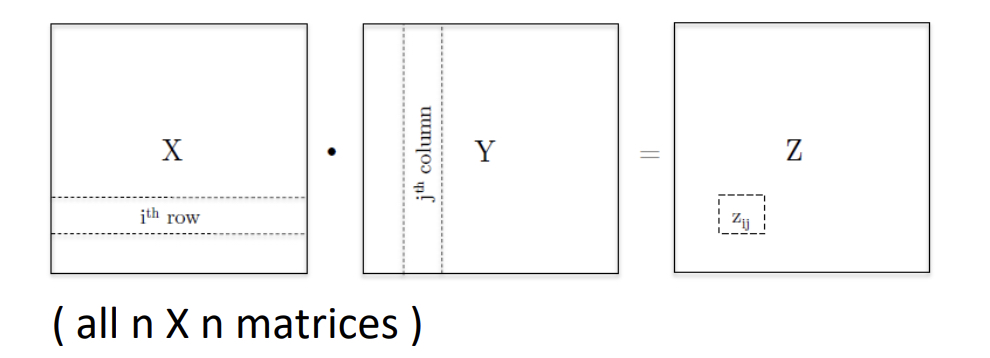
\includegraphics[width=0.6\textwidth]{4.jpg}

    Where $z_{ij} = (i^{th}$ row of $X$) * ($j^{th}$ columns of $Y$)

    $= \sum_{k=1}^{n}X_{ik}*Y_{kj}$ Note: input size = $\theta(n^2)$
\end{center}

\newpage
For example (n = 2):

\vspace{11pt}
\begin{center}
    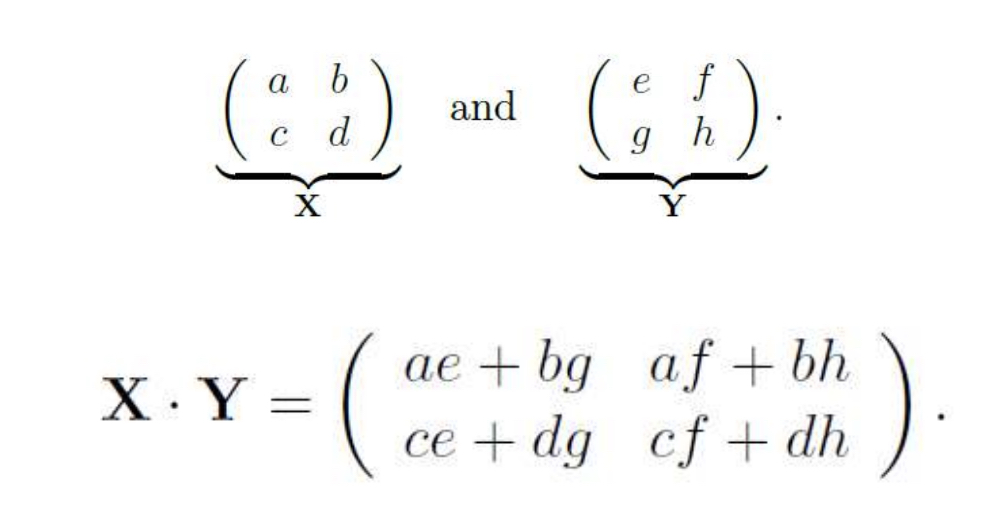
\includegraphics[width=0.5\textwidth]{5.jpg}
\end{center}
\vspace{11pt}

A Straightforward, Naive Algorithm would be:

Input: $n * n$ integer matrices $X$ and $Y$.

Output: $Z = X * Y$

\vspace{11pt}
\begin{lstlisting}
for i = 1 to n do
    for j = 1 to n do
        Z[i][j] = 0
        for k = 1 to n do
            Z[i][j] = X[i][k] + Y[k][j]
return Z
\end{lstlisting}
\vspace{11pt}

So, what is the asymptotic running time of the straightforward algorithm for matrix multiplication, as a function of dimension $n$? Assume that the addition or multiplication of two matrix entries is a constant-time operation. $\to \Theta(n^3)$.

As a Review of the Divide-and-Conquer Paradigm:
\begin{itemize}
    \item 1) DIVIDE into smaller subproblems
    \item 2) CONQUER subproblems recursively.
    \item 3) COMBINE solutions of subproblems into one for the original problem.
\end{itemize}
\vspace{11pt}

To Apply the Divide and Conquer algorithm to Matrix Multiplication:

Write $X=\begin{pmatrix}
A & B \\
C & D
\end{pmatrix}$ and Y = $X=\begin{pmatrix}
E & F \\
G & H
\end{pmatrix}$, where $A$ through $H$ are all $n/2$ by $n/2$ matrices.

Then, you check $X*Y=\begin{pmatrix}
    AE + BG & AF + BH \\
    CE + DG & CF + DH
\end{pmatrix}$.

A recursive approach would be to compute the 8 necessary products and then do the necessary additions ($\theta(n^2)$ time). Note: The $\theta(n^2)$ time for addition comes from the fact that each block has $n/2*n/2$ entries, so the number of entries per block is $\frac{n^2}{4}$. Each entry requires one addition, so $\frac{n^2}{4}$ additions per block * 4 blocks = $n^2$ additions.

The overall runtime is:

\vspace{11pt}
\begin{center}
    $T(n) \leq 8T(\frac{n}{2})+O(n^2)$
    
    $=\theta(n^3)$
\end{center}
\vspace{11pt}

\textbf{Strassen's Algorithm (1969)}
\vspace{11pt}

Strassen's matrix multiplication algorithm recursively computes only 7 (cleverly chosen) products. You still need to do the necessary (clever) additions + subtractions, which is still $\theta(n^2)$ time. But, it is better than cubic time!

\vspace{11pt}
\begin{center}
    $T(n) \leq 7T(\frac{n}{2})+O(n^2)$
    
    $=\theta(n^{log_27})$
\end{center}
\vspace{11pt}

\begin{center}
    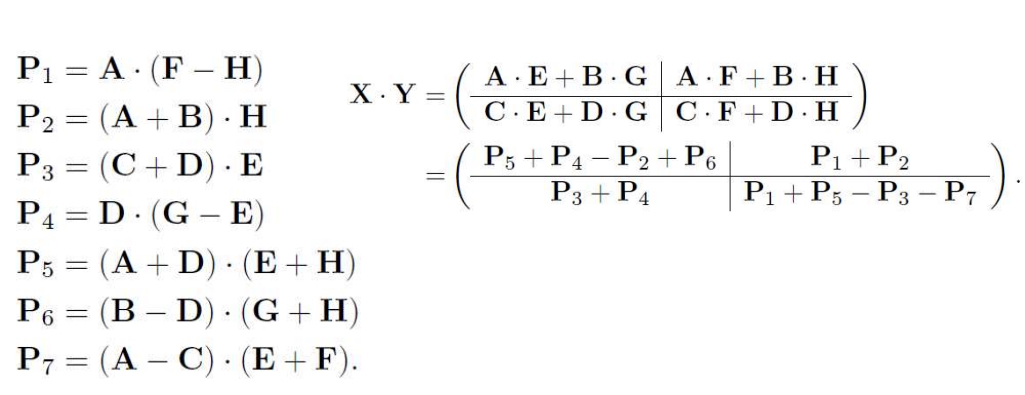
\includegraphics[width=0.6\textwidth]{6.jpg}
\end{center}
\vspace{11pt}

Important topics from this lecture include:
\begin{itemize}
    \item Understanding divide-and-conquer design paradigm.
    \item Understanding how to count inversions in $O(nlogn)$ time.
    \item Understanding the idea of designing a new algorithm by piggybacking on an existing algorithm.
    \item Understanding Strassen's matrix multiplication algorithm.
\end{itemize}
\vspace{11pt}

\vspace{11pt}
\section{Lecture 4 - The Master Method}
\vspace{11pt}

The goal of this lecture is to present a "black-box" method for determining the running time or recursive algorithms. By plugging in a few key characteristics of the algorithm, we can pop out an upper bound on the algorithm's running time.

\vspace{11pt}
\subsection{Integer Multiplication Revisited}
\vspace{11pt}

It is true that potentially useful algorithmic ideas often need mathematical analysis to evaluate. Remember from lecture 1 the grade school multiplication algorithm? It uses $\theta(n^2)$ operations to multiply two $n$-digit numbers.

A recursive approach is to write

\myeq{x=10^{n/2}a+b, y=10^{n/2}c+d}

where [a, b, c, d] are $\frac{n}{2}$ digit numbers. The first algorithm uses this to recursively compute $ac,ad,bc,bd$, then compute ($*$) in the obvious way.

Let $T(n)$ be the maximum number of operations this algorithm needs to multiply two $n$-digit numbers.

Recurrence: We want to express $T(n)$ in terms of running time of recursive calls.

Base Case: $T(1)\leq$ a constant.

For all $n > 1$,

\myeq{T(n) \leq 4T(\frac{n}{2})+O(n)}

However, a better recursive algorithm is the Karatsuba Algorithm, where you recursively compute $ac,bd,(a+b)(c+d)$ where $ad+bc=((a+b)(c+d))-bd-ac$

The new recurrence still has a base case of $T(1) \leq $ a constant. Yet, for $n > 1$, the new running time can be expressed as

\myeq{T(n) \leq 3*T(\frac{n}{2})+O(n)}

\begin{aside}
\textbf{Note}: The $O(n)$ for each recursive level represents the work done outside of the recursive calls. Specifically, this includes additions and subtractions (i.e., to calculate (a+b)(c+d) and then find ad + bc). This includes several operations of n-bit or n/2 bit numbers, each taking linear $O(n)$ time.

Additionally, shifting and combining is also included in this upper bound, where once the three recursive multiplications are complete, the results must be shifted (multiplied by powers of the base) and added together to form the final product. Bit-shifting and adding these results also takes $O(n)$ time.
\end{aside}

\vspace{11pt}
\subsection{The Master Method}
\vspace{11pt}

Traditionally, it was hard to see the exact performance boost from Karatsuba multiplication over the elementary method, but the master method provides a "black box" for solving these types of recursive problems. \textbf{An assumption for recursive problems is that all subproblems have equal size}.

In the Recurrence format, it is assumed that the base case is $T(n) \leq $ a constant for all sufficiently small $n$.

For all larger $n$:

\myeq{T(n) \leq aT(\frac{n}{b}) + O(n^d)}

where
\begin{itemize}
    \item $a = $ number of recursive calls ($\geq 1$).
    \item $b = $ input size shrinkage factor ($>1$).
    \item $d = $ exponent in running time of "combine step" $( \geq 0$).
\end{itemize}
\vspace{11pt}

\begin{aside}
    Note that $a,b,d$ are all independent of $n$.
\end{aside}
\vspace{11pt}

\newpage
Formally, the master method is defined as

\vspace{11pt}
\begin{center}
    $T(n) = \begin{cases} 
    O(n^d \log n) & \text{if } a = b^d \text{ (Case 1)} \\
    O(n^d) & \text{if } a < b^d \text{ (Case 2)} \\
    O(n^{\log_b a}) & \text{if } a > b^d \text{ (Case 3)}
    \end{cases}$    
\end{center}
\vspace{11pt}

\begin{aside}
    Note that in Case 3, the base matters in the logarithm, but same is not true in Case 1.
\end{aside}
\vspace{11pt}

Six example problems using the Master Method are presented in a worksheet distributed in class. This worksheet will be located in the Brightspace course or in my folder for this topic and will not be included in this document.

\vspace{11pt}
\subsection{Proof of the Master Method}
\vspace{11pt}

\textbf{Preamble}
\vspace{11pt}

Assume: Recurrence is
\begin{itemize}
    \item I. $T(1) \leq c$ (for some constant $c$ and small input size $n$)
    \item II. $T(n) \leq aT(n/b) + cn^d$ (we know that $cn^d$ should be bounded above $O(n^2)$.
\end{itemize}
\vspace{11pt}
And $n$ is a power of $b$. The general case is similar, but more tedious. Additionally, let $n = b^k$, and similarly, $k = log_bn$.

Idea: Generalize MergeSort analysis (i.e., use a recursion tree).

\vspace{11pt}
\textbf{A Quiz}: What is the pattern? Fill in the blanks in the following statement: at each level $j = 0, 1, 2, \dots$ of the recursion tree, there are [blank] subproblems, each operating on a subarray of length [blank].

$\to a^j$ and $\frac{n}{b^j}$

\vspace{11pt}
\begin{aside}
    Let $a^j$ be the number of recursive calls per each level, and on the last level, $a^k$ is the number of leaves. Meanwhile, $log_bn + 1$ is the number of levels. $n/b^j$ is the size of the subarray at each level $j$.
\end{aside}
\vspace{11pt}

\textbf{Recursion Tree}

\vspace{11pt}
\begin{center}
    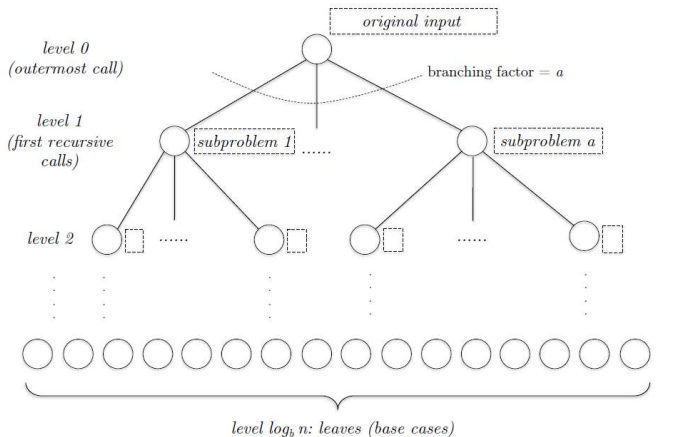
\includegraphics[width=0.5\textwidth]{7.png}
\end{center}

\newpage
\textbf{Level (j)}: $0,1,2,\dots,j,\dots,log_bn$ where $k = log_bn$, so $k+1$ levels.

\textbf{Sub-Problems}: $a^0, a^1, a^2, \dots, a^j, \dots, a^{log_bn} = a^k$.

\textbf{Input Size}: $n/b^0, n/b^1,n/b^2, \dots, n/b^j, \dots, n/b^{log_bn}=n/b^k$. 

\vspace{11pt}
\begin{aside}
    At the last level, the input size of each subproblem is $=n/b^k=1$. Multiplying both sides by $b^k$ gives $n=b^k$, and from this we get $k=log_bn$.
\end{aside}
\vspace{11pt}

Remember, at each level, there are $a^j$ sub-problems (nodes) and $\frac{n}{b^j}$ elements per subarray.

From this information, we can calculate the work at each level and thus, the total work:

Work at a single level:
\vspace{11pt}
\begin{center}
    $lvl(j)\leq c(\frac{n}{b^j})d*a^j$ sub-problems

    Simplifying: $lvl(j) \leq c*a^j*\frac{n^d}{b^{jd}}$

    $lvl(j) \leq c*n^d*(\frac{a}{b^d})^j$
\end{center}
\vspace{11pt}

Given this amount of work at a single level, we can calculate the total amount of work:

\vspace{11pt}
\begin{center}
    total work $\leq \Sigma_{j=0}^{log_bn}c*a^j*(\frac{n}{b^j})^d$

    Simplifying: total work $\leq c*n^d *\Sigma_{j=0}^{log_bn}(\frac{a}{b^d})^j$
\end{center}
\vspace{11pt}

From this, we can see that our upper bound at any level $j$ is $c*n^d*(\frac{a}{b^d})^j$.

Importantly, we can conclude that since the term $b^d$ is in the denominator, the larger its value, the less work per level $j$. Therefore, $b^d$ can be referred to as the \textbf{Rate of Work Shrinkage (RWS)} per sub-problem.

Similarly, since the term $a$ is in the numerator, the larger its value, the more work per level $j$. Therefore, $a$ can be referred to as the \textbf{Rate of Sub-problem Proliferation (RSP)} per sub-problem. 

Now, we will examine three possibilities among the relationship between $a$ and $b^d$.

\vspace{11pt}
\textbf{Case 1 (RSP = RWS)}: When $b^d=a$, the amount of work performed is the same at each recursive level.

\vspace{11pt}
\begin{center}
    $\leq c*n^d *\Sigma_{j=0}^{log_bn}(\frac{a}{b^d})^j$

    $\to c*n^d *\Sigma_{j=0}^{log_bn}(1)^j$
\end{center}
\vspace{11pt}

\textbf{Case 2 (RWS < RSP)}: When $a < b^d$, the amount of work performed decreases with the recursion level $j$.

\vspace{11pt}
\textbf{Case 3 (RSP > RWS)}: When $a > b^d$, the amount of work performed increases with recursion level $j$.

\newpage

\begin{center}
\begin{tabular}{|c|c|c|l|}
    \hline
    Case & Relationship & Big-O & Significance \\ \hline
    1 & $a=b^d$ & $O(n^d \log n)$ & Same amount of work each level \\ \hline
    2 & $a < b^d$ & $O(n^d)$ & Work decreases at each level (Root heavy) \\ \hline
    3 & $a > b^d$ & $O(n^{\log_b a})$ & Work increases at each level (Leaf heavy) \\ \hline
\end{tabular}
\end{center}
\vspace{11pt}

Now, let's examine the math behind each case more closely:

\vspace{11pt}
\textbf{Case 1 ($a=b^d$)}:

\vspace{11pt}
\begin{center}
    $\leq c*n^d *\Sigma_{j=0}^{log_bn}(\frac{a}{b^d})^j$

    where $\frac{a}{b^d}$ is $1$ for all $j$.

    Therefore, $\leq c *n^d(log_bn+1) = O(n^dlogn)$.
\end{center}
\vspace{11pt}

Before looking at Case 2 and Case 3, let's understand some basic sum facts:

\vspace{11pt}
\begin{center}
    $s = 1 + r+r^2+ \dots + r^k$

    $sr = r + r^2 + r^3 + \dots + r^k + r^{k+1}$

    $s-sr = s(1-r)=1-r^{k+1}$
    
    $s = \frac{1-r^{k+1}}{1-r}$
\end{center}
\vspace{11pt}

Now, let's look at two different cases of $r$:
\vspace{11pt}

$r < 1$ is a constant:

\vspace{11pt}
\begin{center}
   $s \leq \frac{1}{1-r}$ is an upper bound where $r$ is a constant.

  \textbf{The first term dominates}.
\end{center}
\vspace{11pt}

$r > 1$ is a constant:

\vspace{11pt}
\begin{center}
    $s=\frac{r^{k+1}-1}{r-1} < \frac{r^{k+1}}{r-1} = r^k*\frac{r}{r-1}$

    $\frac{r}{r-1} = \frac{(r-1)+1}{r-1}$

    $r^k(\frac{r-1}{r-1}+\frac{1}{r-1}) \leq r^k(1+\frac{1}{r-1})$
    
    \textbf{The last term dominates}.
\end{center}
\vspace{11pt}

\begin{aside}
    \textbf{Note:} Both $\frac{1}{1-r}$ and $1+\frac{1}{r-1}$ are independent of $k$
\end{aside}
\vspace{11pt}

\textbf{Case 2 ($a < b^d$)}:

\vspace{11pt}
\begin{center}
    total work $\leq c*n^d*\Sigma_{j=0}^{log_bn}(\frac{a}{b^d})^j$

    $\frac{a}{b^d}$ is $r < 1$ and $\Sigma_{j=0}^{log_bn}r^j \leq$ a constant $\frac{1}{1-r}$.

    $=O(n^d)$.

    The total work is dominated by the top level.
\end{center}
\vspace{11pt}

\textbf{Case 3 ($a > b^d$)}:

\vspace{11pt}
\begin{center}
    total work $\leq c*n^d*\Sigma_{j=0}^{log_bn}(\frac{a}{b^d})^j$

    $\frac{a}{b^d}$ is $r > 1$ and $\Sigma_{j=0}^{log_bn}r^j \leq$ a constant $(1+\frac{1}{1-r}) * $ the largest term $r^k$.

    $=O(n^d*(\frac{a}{b^d})^{log_bn})$

    Note: $b^{-dlog_nb} = (b^{log_nb})^{-d}=n^{-d}$ since $b^{log_bn}=b^k$ and $b^k=n$.

    So, $(*) =O(a^{log_bn}) = O(\# \space leaves)$.

    $=O(n^{log_ba})$

    The total work is dominated by the bottom level.
\end{center}
\vspace{11pt}

\subsection{Summary: The Master Method}
\vspace{11pt}

If $T(n) \leq aT(\frac{n}{b})+O(n^d)$

then:

\vspace{11pt}
\begin{center}
    $T(n) = \begin{cases} 
    O(n^d \log n) & \text{if } a = b^d \text{ (Case 1)} \\
    O(n^d) & \text{if } a < b^d \text{ (Case 2)} \\
    O(n^{\log_b a}) & \text{if } a > b^d \text{ (Case 3)}
    \end{cases}$    
\end{center}
\vspace{11pt}

It is important to apply the master method to determine the running time of recursive algorithms. Additionally, you should apply the intuition to understand the master method.

\vspace{11pt}
\section{Lecture 5 - Quick Sort}
\vspace{11pt}

\boldsecbottom{Why QuickSort?}

In homework two, we implemented merge sort, which was $O(nlogn)$, so why do we need another sorting algorithm?

The truth is that both Merge Sort and QuickSort are both widely used.

QuickSort is definitely a "greatest hit" algorithm. In other words, it is considered one of the top algorithms ever derived. It is also very prevalent in practice. 

The analysis is also beautiful, too. We will skip it in this class, however.

In QuickSort, we do not use merge, so there is less extra space. Instead of taking two arrays to merge, \textbf{QuickSort swaps two elements}. On average, it is an $O(nlogn)$ algorithm that works in place (i.e., minimal extra memory needed).

We can also use QuickSort to introduce a randomization algorithm.

\newpage
\subsection{QuickSort Overview}
\vspace{11pt}

\boldsecbottom{The Sorting Problem}

We have unsorted data, and we want to sort it from the smallest element to the largest element. It is pretty straight forward.

Given an input of an array of $n$ numbers, unsorted, we want the output to be the same numbers, sorted in increasing order.

\vspace{11pt}
$[4,2,6,1, \dots] \to [1,2,3,4,5,6,7,8]$.

\vspace{11pt}
We will assume that all array entries are \textbf{distinct}. However, in QuickSort, there could be a possibility that two elements have an identical value. We need to extend QuickSort to handle duplicate entries.

\boldsec{Partitioning Around a Pivot}

The key idea of QuickSort is to have a partition array around a pivot array. We pick a random element of the array. Then, we want to rearrange the array so that the left of the pivot is less than the pivot and that the right of the pivot is greater than the pivot. Therefore, this puts the pivot in its "rightful position."

\vspace{11pt}
$[3,8,2,5,1,4,7,6] \to [2,1,3,6,7,4,5,8]$

\vspace{11pt}

If we choose $3$ as the pivot, then all elements to the left of it are less than the pivot and all the elements to the right of it are greater than it.

\vspace{11pt}
What is the runtime of a partition? $O(n)$.

\boldsec{Two Cool Facts About Partition}

\begin{itemize}
    \item Linear $O(n)$ time, no extra memory.
    \item Reduces problem size. After the partition is in the right position, there are two sub-arrays that are reduced in size. Ideally, they are half and half, but this might not be true as they may not be equal sizes.
\end{itemize}

\boldsec{QuickSort: High-Level Description}

\texttt{QuickSort(Array A, length n)}

The base case is if $n = 1$, then return since its already sorted. Then, we choose $p$, a pivot value using ChoosePivot($A$, $n$). We then partition $A$ around $p$. Then recursively sort the first and second part.

\myeq{[<p,p,>p]}

We keep doing this until the sub-array size is one.

\boldsecbottom{MergeSort vs. QuickSort}

A big similarity is that both algorithms use a divide-and-conquer approach.  

However, for Quick Sort, the first step is partitioning (pivot and put it in correct position) and then divide, and then conquer recursively. There is also \textbf{no} \textbf{combine} step for Quick Sort. In fact, \textbf{recursive calls occur after partitioning}.

\boldsec{Three Questions}
\begin{itemize}
    \item How to implement the partition subroutine?
    \item How to choose the pivot element?
    \item What is the running time of QuickSort?
\end{itemize}

\vspace{11pt}
\subsection{QuickSort Implementation}
\vspace{11pt}

\boldsecbottom{The Easy Way Out [Naive Approach]}

What is the "easiest" way to complete the partitioning?

\myeq{[3,8,2,5,1,4,7,6]}

We can choose the first element in the array as the pivot. In this case: 3. We then look at the next element, which is 8. Since $8 > 3$, we put 8 at the end. We then get to $2$, put it on the left. Then right, left, right, right, and right for the remaining elements.

This uses $O(n)$ extra memory, making it easy to partition around pivot in $O(n)$.

However, can we do better and get rid of this $O(n)$ extra memory requirement? Yes.

\boldsec{In-Place Implementation}

We still assume that we are going to choose the pivot as the first element of the array. If not, we can swap the pivot with the first element of the array as a pre-processing step.

After choosing a pivot element, the high level idea is:

\myeq{[p, <p, >p, ?]}

We scan through the array once. Invariant means that everything looked at so far is partitioned.

Again, say we have:

\myeq{[3,8,2,5,1,4,7,6]}

We have the pivot element of 3, but everything else to the right is un-partitioned. We have two indices, $i,j$ that initially point to the position right after the pivot. We look at 8, $8 > 3$, we then keep the $i$ here without changing since $i$ indicates the boundary between less than pivot and greater than pivot. However, $j$ moves to point to the element after 8 as un-partitioned.

Now, lets consider 2. Is $2 > 3$, no, its less than 3. So, we have 8 and 2 swap places:

\myeq{[3,2,8, \dots]}

$i$ increases by one to the element after 2. $j$ increases to the element after 8. Now lets consider 5. $5 > 3$, so we keep $i$ in place and move $j$ to the element after 5. Now for the next one $1 < 3$, so we need to swap 1 with the number 8. We then increase $i$ to point to the position after 1 and move j to move to the position after 8 (post swap). 

The rest of the elements are greater and eventually $j$ will point at the very end of the array. 

However, we still need to place the pivot in the correct position. We replace the pivot, 3, with the value at the $i - 1$ index.

\boldsec{Pseudo code for Partition}

\begin{lstlisting}[language=python, breaklines=true]
Partition(A,l,r) # A[l, ..., r]
    p = A[l] 
    i = l + 1
    for j=l+1 to r
        if A[j] < p  # [if A[j] > p, do nothing]
            swap A[j] and A[i]
            i = i + 1
    swap A[l] and A[i-1]
    return i - 1
\end{lstlisting}
\vspace{11pt}

The runtime for this partition is $O(n)$, where $n = r - l + 1$ is the length of the input (sub) array. The reason is that there is $O(1)$ work per array entry. It also clearly works in place (repeated swaps).

\boldsec{Correctness}

Claim: The for loop maintains the invariants:

\begin{itemize}
    \item $A[l+1],..,A[i-2]$ are all less than the pivot.
    \item $A[i], ..., A[j-1]$ are all greater than the pivot.
\end{itemize}
\vspace{11pt}

We can check this by induction. We check $k + 1$ element.

The consequence is that at the end of the for loop, we have an array partitioned around a pivot.

\boldsec{Pseudo code for QuickSort}

Input: Array $A$ of $n$ distinct integers, left and right endpoints $l,r \in [1,2,\dots,n]$.
Post condition: elements of the subarray $A[l],A[l+1],\dots,A[r]$ are sorted from smallest to largest.

\vspace{11pt}
\begin{lstlisting}[language=python, breaklines=true]
if l >= r then # 0 or 1 element subarray
    return
i := ChoosePivot(A,l,r) # To be implemented
swap A[l] and A[i] # make pivot first
j := Partition(A,l,r) # j = new pivot position
QuickSort(A,l,j-1) # recurse on first part
QuickSort(A,j+1,r) # recurse on second part

\end{lstlisting}
\vspace{11pt}

\boldsecbottom{The Importance of a Good Pivot}

What is the running time of QuickSort? It depends on the quality of the pivot.

\boldsec{Naive Implementation of Choose Pivot}

\texttt{ChoosePivot(Naive Implementation)}

Input: array $A$ of $n$ distinct integers, left and right endpoints $l,r \in [1,2,\dots,n]$.

Output: an index $i \in [l,l+1,\dots,r]$.

\vspace{11pt}
\begin{lstlisting}[language=python, breaklines=true]
return l
\end{lstlisting}

\boldsec{Quiz [1]}

What is the running time fo the QuickSort algorithm, with the naive implementation of \texttt{ChoosePivot}, when the $n-$element input array is already sorted.
$\to \Theta(n^2)$.

\vspace{11pt}
Given

\myeq{[1,2,3,4,5,6,7,8]}

If we constantly choose the first element as the partition, we never do any swapping since everything is already sorted. So $n + (n-1) + (n-2) + \dots + 1 = \frac{(1+n)*n}{2} = \Theta(n^2)$ ($\Theta$ to represent a tight bound).

\boldsec{Overkill Implementation of ChoosePivot}

\texttt{ChoosePivot(Overkill Implementation)}

Input: Array $A$ of $n$ distinct integers, left and right endpoints $l, r \in [1,2,\dots,n]$.

Output: an index $i \in [l,l+1,\dots,r]$.

\vspace{11pt}
\begin{lstlisting}[language=python, breaklines=true]
return position of the median element of {A[l],...,A[r]}
\end{lstlisting}

\boldsec{Quiz [2]}

What is the running time of the QuickSort algorithm, with the overkill implementation of ChoosePivot, on an arbitrary $n-element$ input array? Assume that the ChoosePivot subroutine runs in $\Theta(n)$ time.

$\to \Theta(nlogn)$. Using the master method: $T(n) \leq 2T(n/2)+O(n)$. We have $a=2,b=2,d=1$. We have case 1 so $\Theta(nlogn)$.

\boldsec{Random Pivots}

The key question is how to choose pivots? BIG IDEA: RANDOM PIVOTS!

That is, in every recursive call, we choose the pivot randomly (each element equally likely). The hope is that a random pivot is "pretty good" or "often enough".

The intuition is that if we always get a 25-75 split, that is good enough for $O(nlog(n))$ running time. This is a non-trivial exercise proven using a recursion tree. In fact, half of the elements give a 25-75 split or better.

\boldsec{Randomized Algorithm}

A randomized algorithm is one that "flips coins" as it proceeds and can make decisions based on the outcomes of these coin flips. All of the major programming languages include libraries that make it easy to pick random numbers at will, and randomization is a tool that should be in the toolbox of every serious algorithm designer.

As it turns out, there are hundreds of computational problems for which randomized algorithms are faster, more effective, or easier to code than their deterministic counterparts.

\boldsec{Randomized Implementation of ChoosePivot}

\texttt{ChoosePivot(Randomized Implementation)}

Input: Array $A$ of $n$ distinct integers, left and right endpoints $l,r\in[1,2,\dots,n]$.

Output: An index $i \in [l,l+1,\dots,r]$.

\vspace{11pt}
\begin{lstlisting}[language=python, breaklines=true]
Returns: An element of [l,l+1,...,r] chosen uniformly at random    
\end{lstlisting}

\boldsec{Average Running Time of QuickSort}

The QuickSort Theorem states that for every input array of length $n$, the average running time of QuickSort (with random pivots) is $O(nlog(n))$.

Note: This holds for every input, and there are no assumptions on the data. Recall our guiding principle, we only consider for every possible input array and consider the worst case.

The "average" is over random choices made by the algorithm (i.e., the pivot choices).

\boldsec{Sorting Requires $O(nlogn)$ Comparisons}

Theorem 5.5 (Lower Bound for Sorting) states there is a constant $c > 0$ such that, for every $n \geq 1$, every comparison-based sorting algorithm performs at least $c *nlog_2n$ operations on some length$-n$  input array.

However, there are faster sorting strategies under strong assumptions that are not comparison based:
\begin{itemize}
    \item BucketSort
    \item CountingSort
    \item RadixSort
\end{itemize}

\boldsec{Summary}

It is important to understand how to implement QuickSort, especially considering it is a first-ballot hall-of-fame algorithm. It is also important to understand how to apply randomization in an algorithm (i.e. a randomized QuickSort).

Remember that sorting requires $O(nlogn)$ comparisons.













































\end{document}